
% Slideshow, written by Brent Baccala, for a lecture at TJHSST

\documentclass{beamer}
\usetheme{Madrid}

\title{A New Solution to Hydrogen}
\author{Brent Baccala}
\institute{\tt cosine@freesoft.org}
%% \date{February 8, 2023}

\setbeamertemplate{footline}{}
\beamertemplatenavigationsymbolsempty

\usepackage{xcolor}
\usepackage{comment}
\usepackage{graphicx}

\usepackage{tabularx}

\begin{document}


\begin{frame}
\titlepage
\begin{block}{Abstract}
A New Solution to Hydrogen
\end{block}
\end{frame}

\begin{frame}
\begin{exampleblock}{}
\begin{center}
\vskip 20pt
\Huge
Part 1: Schr\"odinger's Equation
\vskip 6pt
\ 
\end{center}
\end{exampleblock}
\end{frame}

\begin{frame}
\frametitle{Force, Field, Potential, Potential Energy}
\end{frame}

\begin{frame}
\frametitle{Hamiltonian Mechanics}
\end{frame}

\begin{frame}
\frametitle{(Time Dependent) Schr\"odinger Equation}
%% 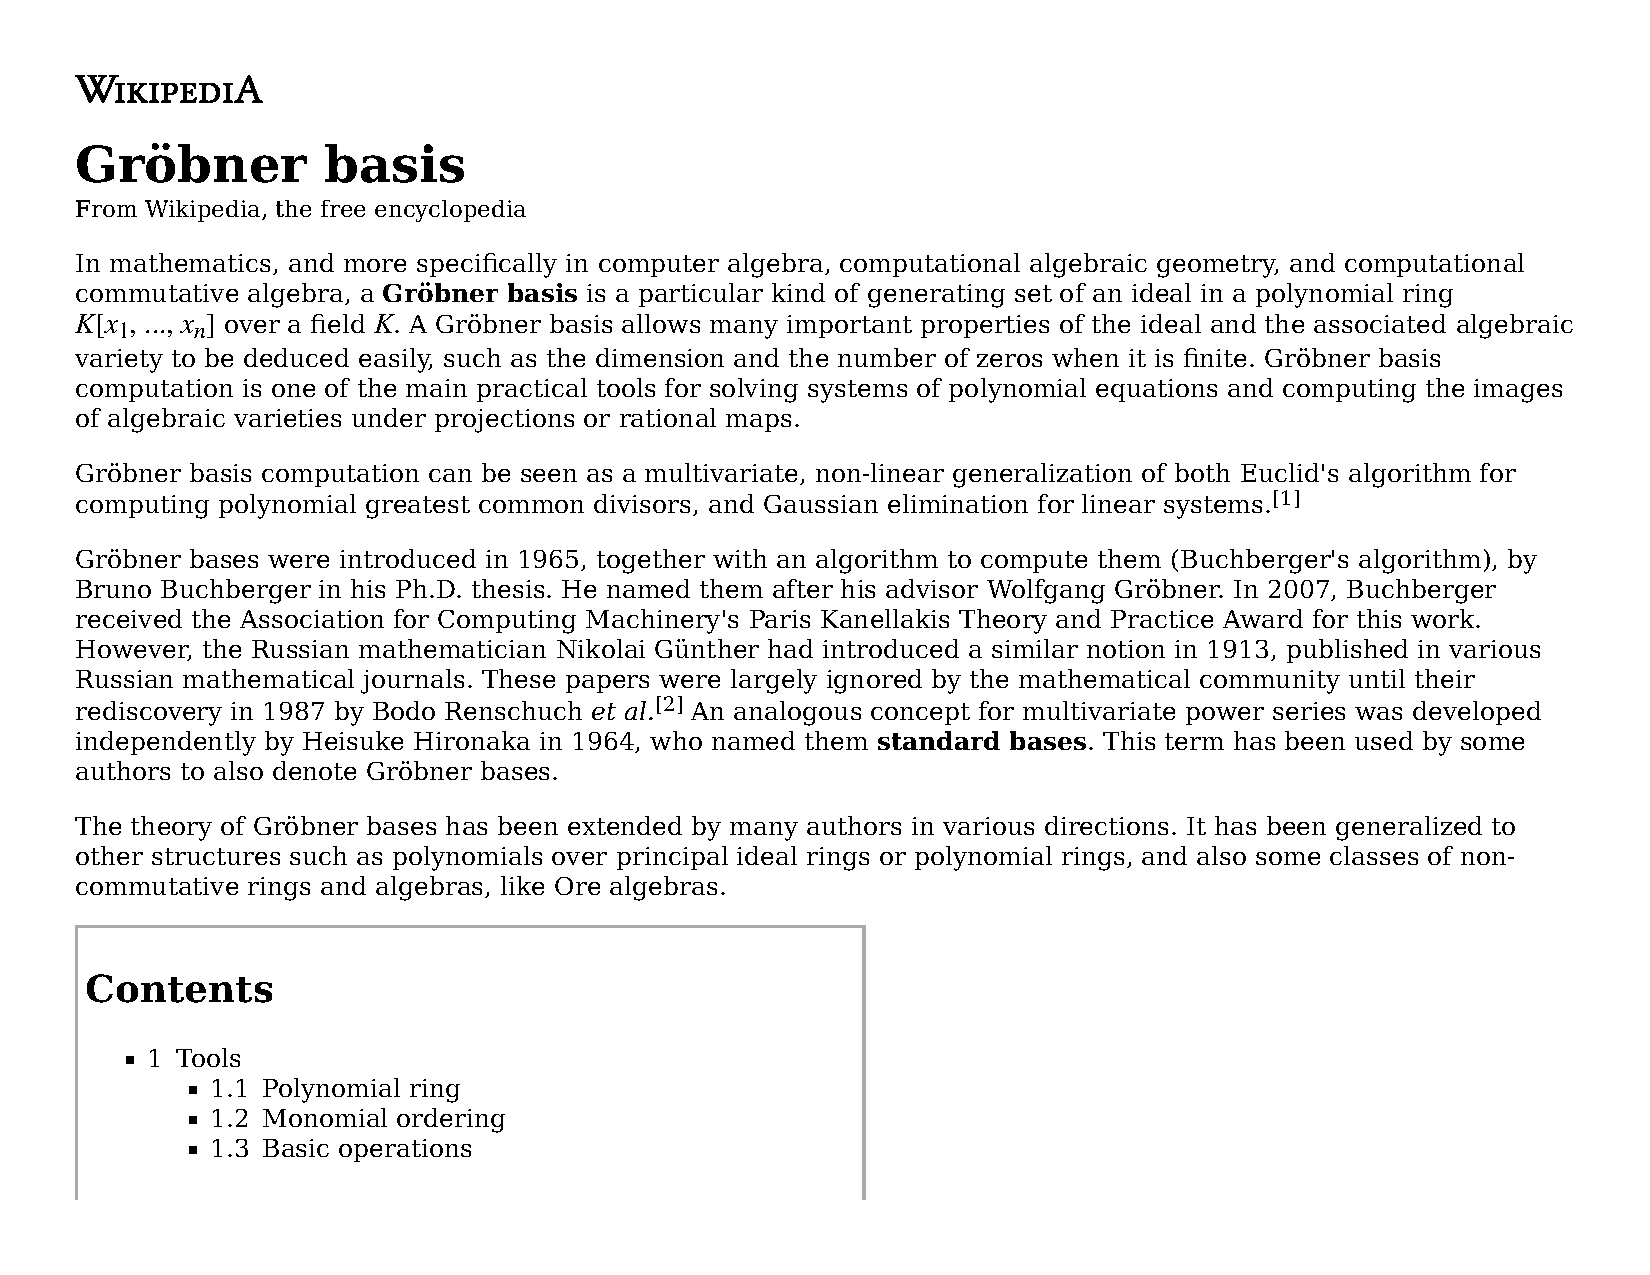
\includegraphics[clip, trim=0in 5.6in 0in 0.75in, width=\textwidth, page=1]{GrobnerBasis.pdf}
%% \includegraphics[clip, trim=0in 6.25in 0in 0.5in, width=\textwidth, page=9]{GrobnerBasis.pdf}
%% \includegraphics[clip, trim=0in 3in 0in 0.5in, width=\textwidth, page=13]{GrobnerBasis.pdf}
\[ H \Psi = i \frac{\delta}{\delta t} \Psi \]
\end{frame}

\begin{frame}
\frametitle{Time Independent Schr\"odinger Equation}
\[ H \Psi = E \Psi \]
\end{frame}

\begin{frame}
\frametitle{Hydrogen Schr\"odinger Equation}
\end{frame}

\begin{frame}
\frametitle{Helium Schr\"odinger Equation}
\end{frame}

\begin{frame}
\frametitle{The Classical Solutions to Hydrogen}
\end{frame}

\begin{frame}
\frametitle{The New Solution to Hydrogen}
\end{frame}

\begin{frame}
\frametitle{Bessel Functions}
\end{frame}

\begin{frame}
\begin{exampleblock}{}
\begin{center}
\vskip 20pt
\Huge
Part 2: Differential Algebra
\vskip 6pt
\ 
\end{center}
\end{exampleblock}
\end{frame}

\begin{frame}
\frametitle{Classical Galois Theory}
\end{frame}

\begin{frame}
\frametitle{Differential Galois Theory}
\end{frame}

\begin{frame}
\frametitle{Picard-Vessiot Theory}
\end{frame}

\begin{frame}
\begin{exampleblock}{}
\begin{center}
\vskip 20pt
\Huge
Part 3: Moving the Research Project Forward
\vskip 6pt
\ 
\end{center}
\end{exampleblock}
\end{frame}

\begin{frame}
\frametitle{Methods of Solving Systems of Polynomial Equations}
\begin{itemize}
\item Primary Decomposition with Gr\"obner Bases
\item Homotopy Continuation
\item Numerical Optimization (Levenburg-Marquardt)
\end{itemize}
\end{frame}

\begin{frame}
\frametitle{The Euclidean Distance Function}
\end{frame}

\begin{frame}
\frametitle{Use of Large Language Models in Software Development}
\end{frame}

\end{document}
